\subsubsection{Exception package}

\paragraph{Package: exceptionPackage}This package contains all MatFlowExceptions.

\class{Exception}

\begin{figure}[H]
        \centerline{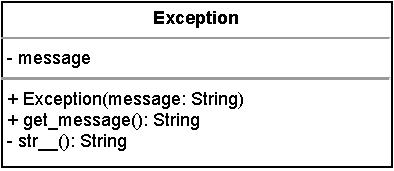
\includegraphics[scale=1]{res/Klassen/Exception.pdf}}
        \caption{Exception class from class diagram}
\end{figure}

This is the native Python exception package. See \url{https://docs.python.org/3/tutorial/errors.html} 
for more information on usage and best practices.

\class{MatFlowException}

\begin{figure}[H]
        \centerline{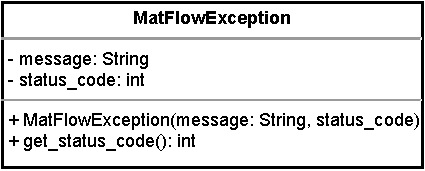
\includegraphics[scale=1]{res/Klassen/MatFlowException.pdf}}
        \caption{MatFlowException class from class diagram}
\end{figure}

This is the MatFlow parent exception from which all the specified exceptions inherit. It adds more functionality to 
a standard exception through the exception's status code and function which gets the status code. This is important for our
\nameref{API}.
\begin{methodenv}{Constructor}
\method{MatFlowException(message: String, status\texttt{\_}code: int): MatFlowException}
\smallPara{Parameters}
\begin{itemize}
	\item{message:}
	The message that is displayed when the exception is thrown. Native to the parent class but not relevant to application,
    nevertheless intriguing when extending this application 
    \item{status\texttt{\_}code:}
	The status code representing the thrown exception
\end{itemize}

\method{get\texttt{\_}status\texttt{\_}code(): int}
gets the status code

\end{methodenv}


\class{UserExistsException}

\begin{figure}[H]
        \centerline{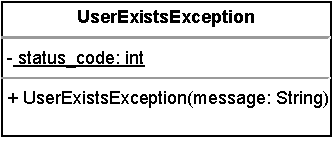
\includegraphics[scale=1]{res/Klassen/UserExistsException.pdf}}
        \caption{UserExistsException class from class diagram}
\end{figure}

This is an exception that is thrown when a user does not exist.
\begin{methodenv}{Constructor}

\method{UserExistsException(message : String)}
\smallPara{Parameters}
\begin{itemize}
    \item{message:}
    The message that is displayed when this exception is thrown.
\end{itemize}

\end{methodenv}

\class{DoubleTemplateNameException}

\begin{figure}[H]
    \centerline{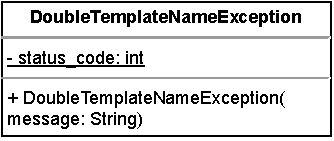
\includegraphics[scale=1]{res/Klassen/DoubleTemplateNameException.pdf}}
    \caption{DoubleTemplateNameException class from class diagram}
\end{figure}

This is an exception that is thrown when the desired template name already exists.
\begin{methodenv}{Constructor}

\method{DoubleTemplateNameException(message : String)}
\smallPara{Parameters}
\begin{itemize}
    \item{message:}
    The message that is displayed when this exception is thrown.
\end{itemize}
\end{methodenv}


\class{InvalidDagFileException}

\begin{figure}[H]
    \centerline{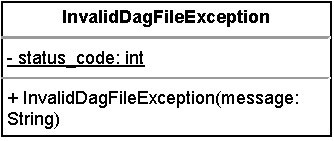
\includegraphics[scale=1]{res/Klassen/InvalidDagFileException.pdf}}
    \caption{InvalidDagFileException class from class diagram}
\end{figure}

This is an exception that is thrown when the dag definition file is not correct (when dag file is finished coding).
\begin{methodenv}{Constructor}

\method{InvalidDagFileException(message : String)}
\smallPara{Parameters}
\begin{itemize}
    \item{message:}
    The message that is displayed when this exception is thrown.
\end{itemize}
\end{methodenv}


\class{DoubleWorkflowInstanceNameException}

\begin{figure}[H]
    \centerline{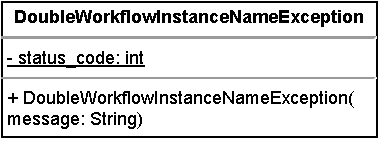
\includegraphics[scale=1]{res/Klassen/DoubleWorkflowInstanceNameException.pdf}}
    \caption{DoubleWorkflowInstanceNameException class from class diagram}
\end{figure}

This is an exception that is thrown when the desired workflow instance name already exists.
\begin{methodenv}{Constructor}

\method{DoubleWorkflowInstanceNameException(message : String)}
\smallPara{Parameters}
\begin{itemize}
    \item{message:}
    The message that is displayed when this exception is thrown.
\end{itemize}
\end{methodenv}


\class{EmptyConfigFolderException}

\begin{figure}[H]
    \centerline{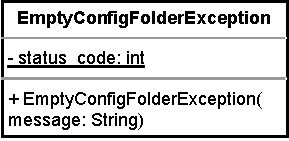
\includegraphics[scale=1]{res/Klassen/EmptyConfigFolderException.pdf}}
    \caption{EmptyConfigFolderException class from class diagram}
\end{figure}

This is an exception that is thrown when the config folder is empty, meaning that no config can be selected.
\begin{methodenv}{Constructor}

\method{EmptyConfigFolderException(message : String)}
\smallPara{Parameters}
\begin{itemize}
    \item{message:}
    The message that is displayed when this exception is thrown.
\end{itemize}
\end{methodenv}


\class{WorkflowInstanceRunningException}

\begin{figure}[H]
    \centerline{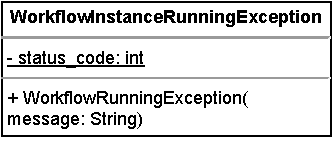
\includegraphics[scale=1]{res/Klassen/WorkflowInstanceRunningException.pdf}}
    \caption{WorkflowInstanceRunningException class from class diagram}
\end{figure}

This is an exception that is thrown when the workflow instance is already running.
\begin{methodenv}{Constructor}

\method{WorkflowInstanceRunningException(message : String)}
\smallPara{Parameters}
\begin{itemize}
    \item{message:}
    The message that is displayed when this exception is thrown.
\end{itemize}
\end{methodenv}

\class{UnrepresentableDagException}

\begin{figure}[H]
    \centerline{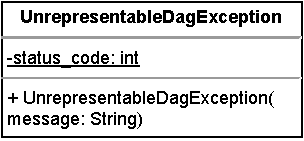
\includegraphics[scale=1]{res/Klassen/UnrepresentableDagException.pdf}}
    \caption{UnrepresentableDagException class from class diagram}
\end{figure}

This is an exception that is thrown when the dag cannot be previewed(when dag file editing is in progress (JUST preview)).
\begin{methodenv}{Constructor}

\method{UnrepresentableDagException(message : String)}
\smallPara{Parameters}
\begin{itemize}
    \item{message:}
    The message that is displayed when this exception is thrown.
\end{itemize}
\end{methodenv}